One AlphaSense NO2 sensor was tested against the EPA reference.  It was 2 months old at the time of installation, and ran for 21 days (from 5/23 - 6/13 2016).  This test gave 30,150 minute resolved samples.


\subsection{Pre-processing}

The AlphaSense NO2 raw data has similar concerns to its CO counterpart-- it appears heavily `quantized' based on the temperature regime it is in.  The NO2 values were much further off than the CO values though, using the raw calculation.  

\begin{marginfigure}
 	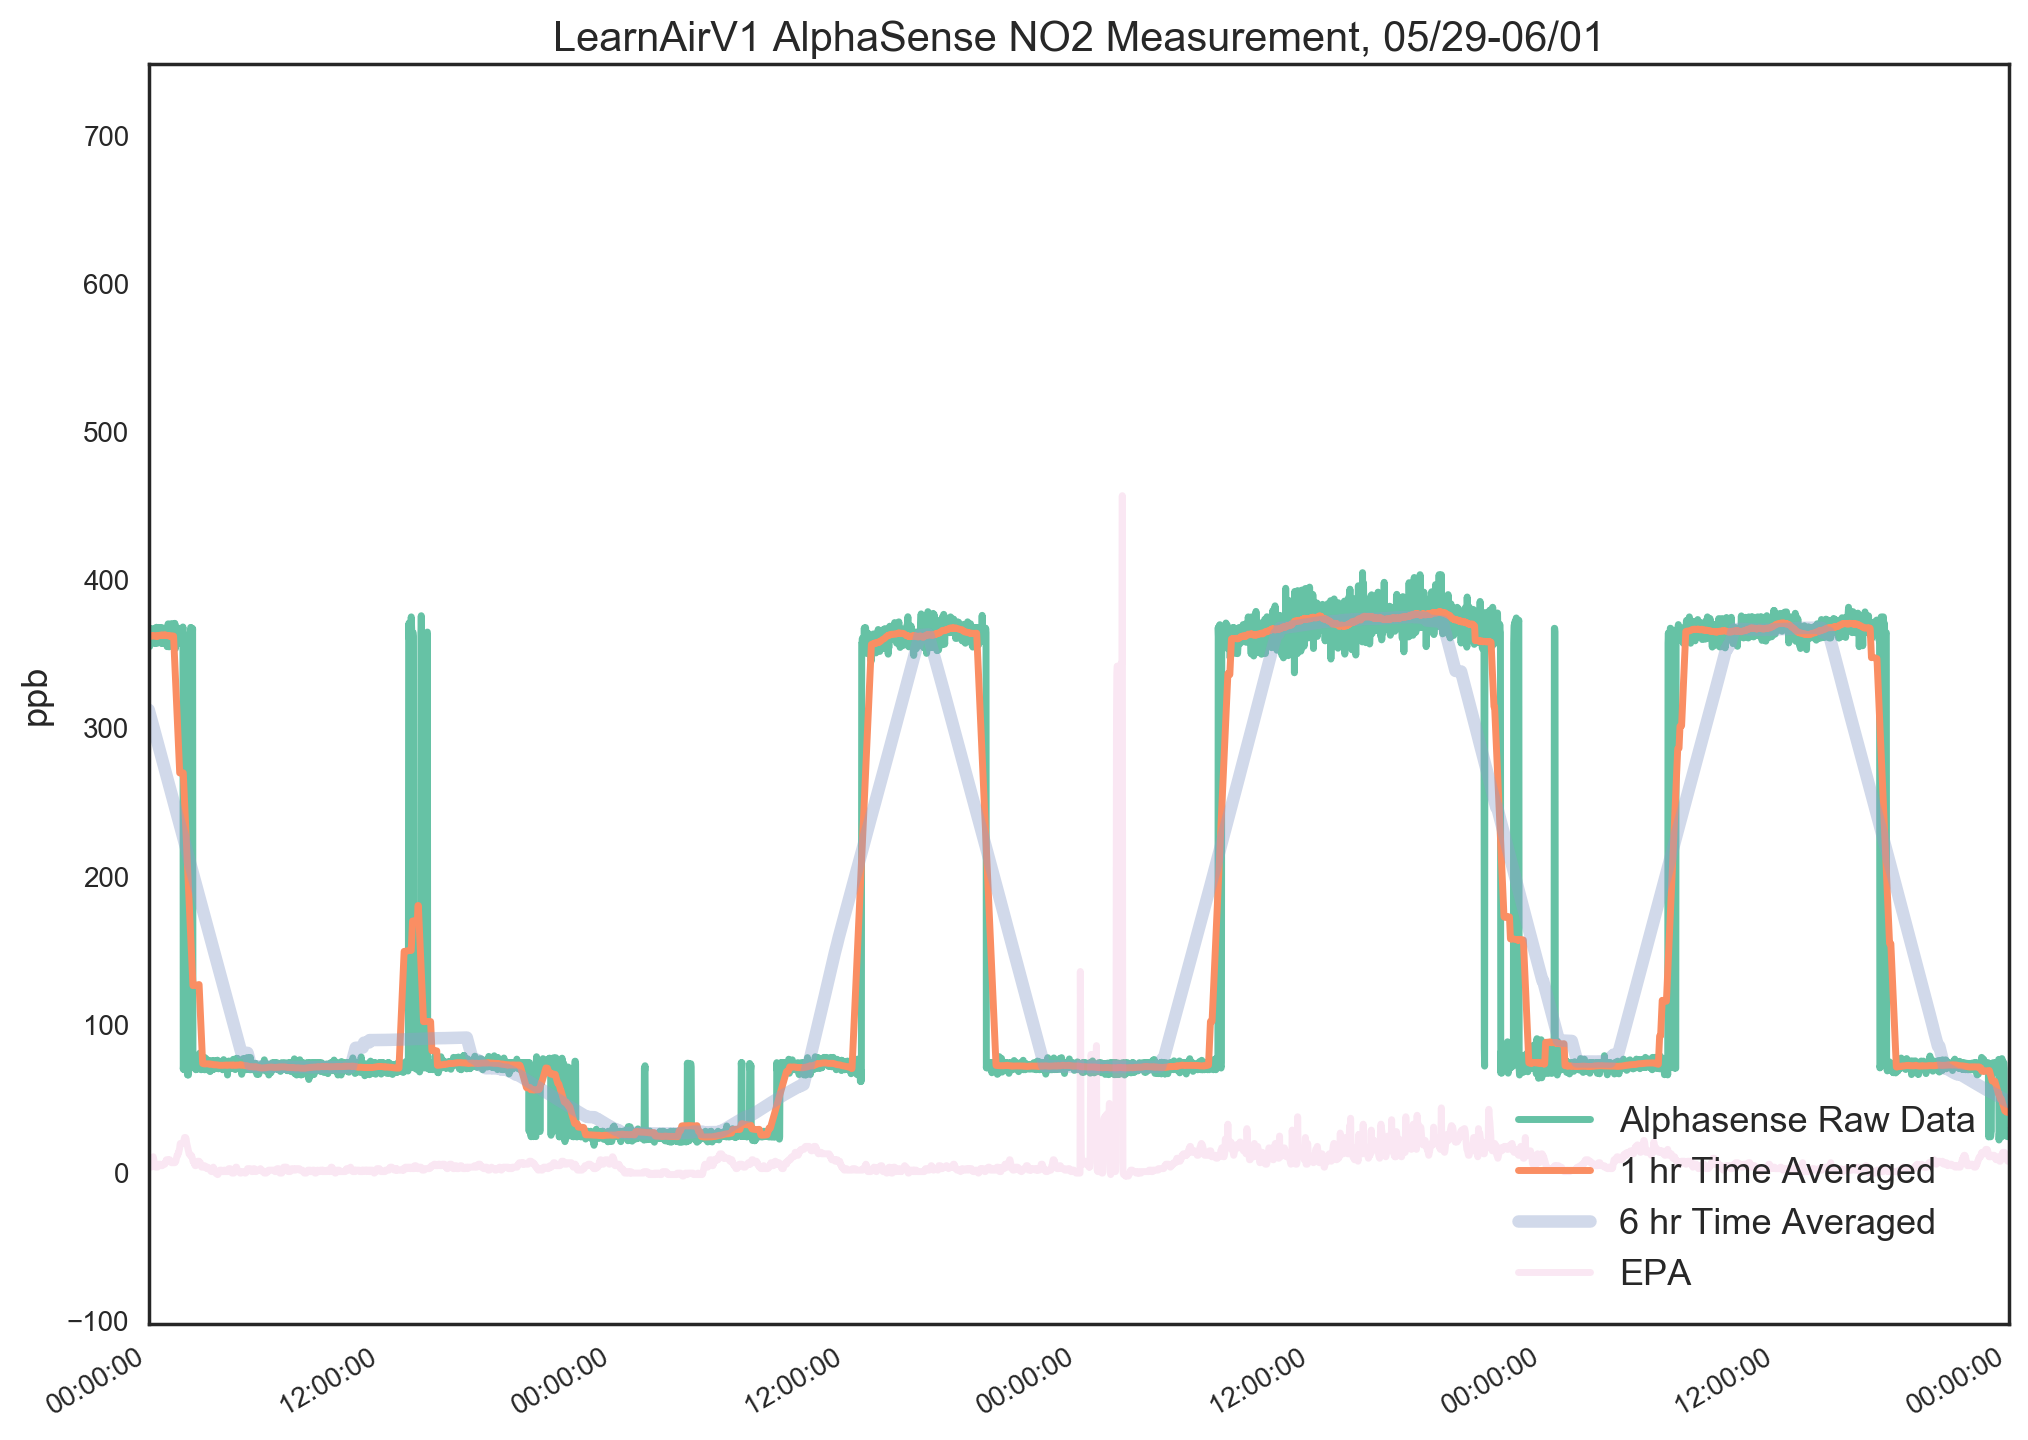
\includegraphics[width=\textwidth]{figs/as_no2_raw_zoomed}               
 	 \caption{AlphaSense NO2 Raw Data Zoomed}
  	\label{fig:as_no2_raw_zoomed}
\end{marginfigure}

Many techniques were used to tighten up the calibration after applying the initial datasheet equation and values, some of which greatly alter the variation, but at the end of the day a milder form was chosen based on scaling the electrode offsets.  The final results can be seen in Figure \ref{fig:as_no2_with_10_accuracy_zoomed}.  

\subsection{Machine Learning}

NO2 has some of the smallest variations of the pollutants we looked at.  To assess its accuracy, 10\% of its full scale value was used as a tolerance-- this worked out to a very tight tolerance of $\pm$26.25 ppb.  With this tolerance in place, our parameterized search of C = [0.001, 0.1, 10, 1000] and penalty-type=['L1', 'L2'] with a 2-fold cross-validation yielded an optima set of L1 penalty with C = 1000.    

\begin{figure}[htb]
 	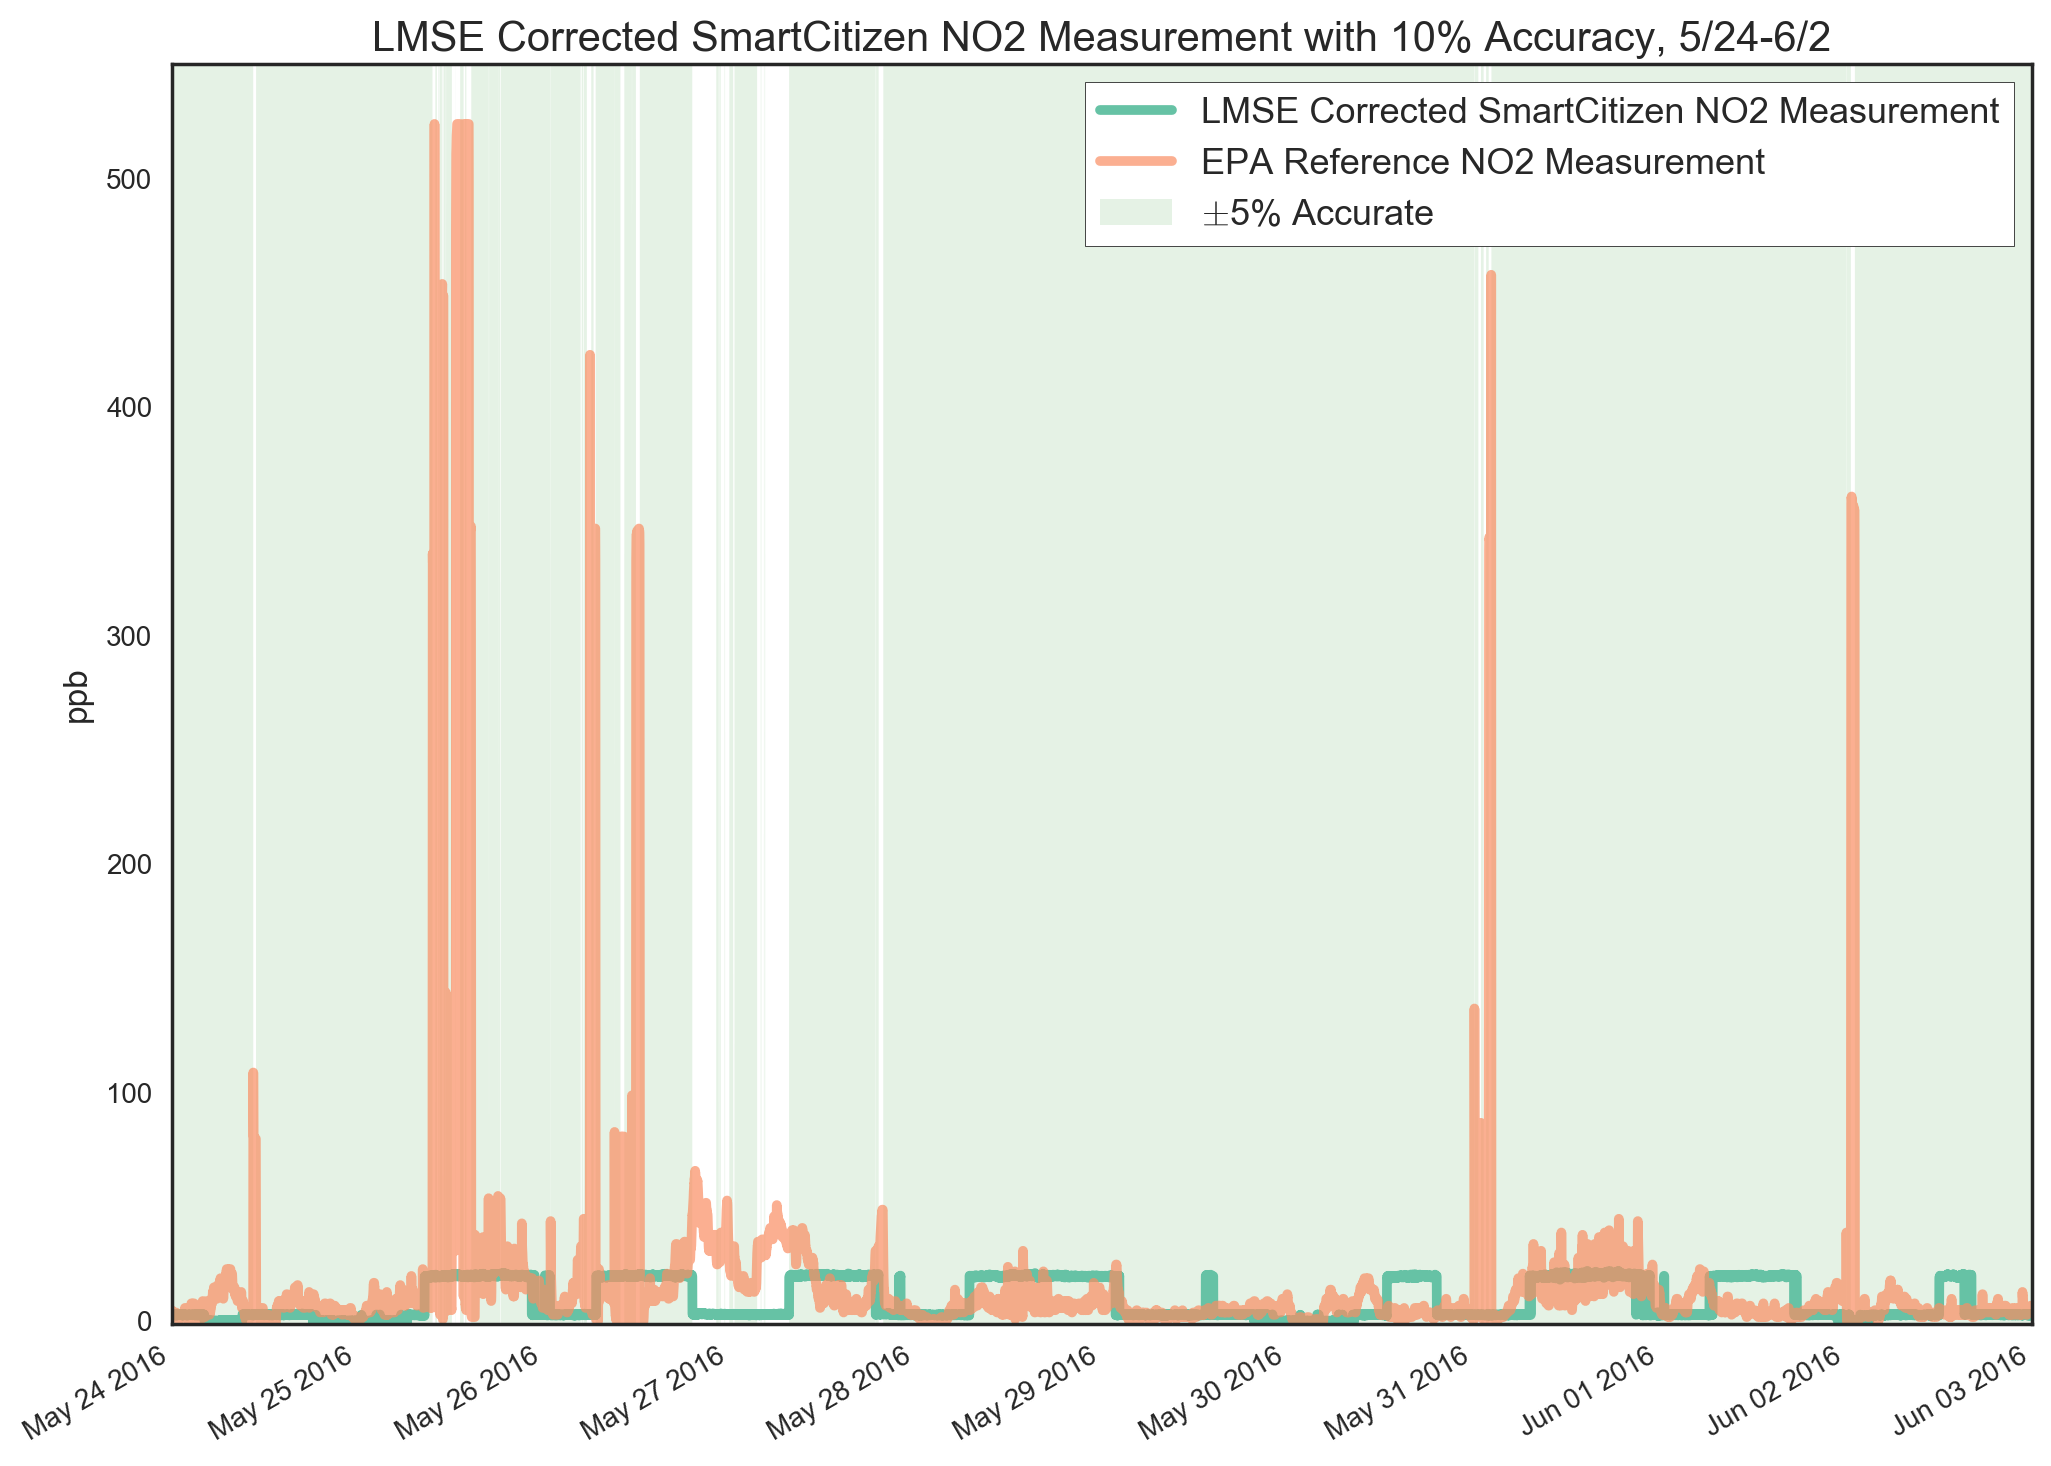
\includegraphics[width=\textwidth]{figs/as_no2_with_10_accuracy_zoomed}               
 	 \caption{AlphaSense NO2 with 10\% Accuracy Threshold}
  	\label{fig:as_no2_with_10_accuracy_zoomed}
\end{figure}


Even with this extremely tight tolerance, we can see in Table \ref{tab:as_no2_error_rates} that we have very low average error rates in all conditions, though our variability dramatically increases for the chunked cases.  In conjunction with the ROC graphs of Figure \ref{fig:as_no2_10_roc} we can see that our seasonal predictive power is quite poor.  This isn't unexpected, as this test (a three week test) was one of the shortest performed.


\begin{table}
\centering
\begin{tabular}{|c|c|c|c|c|}
\toprule
\multicolumn{5}{|c|}{Error Rates for AlphaSense NO2 with Logistic Regression} \\
&\multicolumn{2}{|c|}{all features} & \multicolumn{2}{|c|}{top 15 features} \\
&shuffled & chunked & shuffled & chunked \\
avg & 0.03 & 0.06 & 0.04 & 0.04 \\
min & 0.03 & 0.05 & 0.03 & 0.01 \\
max & 0.03 & 0.14 & 0.04 & 0.14 \\
\bottomrule
\end{tabular}
\label{tab:as_no2_error_rates}
\caption{Error Rates for Predicting AlphaSense NO2 Accuracy with Logistic Regression}
\end{table}



\begin{margintable}
\centering
\offinterlineskip
\hspace*{-5cm}\raisebox{-4cm}[0pt][0pt]{\rotatebox[origin=c]{90}{\parbox[c][0pt][c]{3cm}{\textbf{Actual Values}\\[20pt]}}}\par
\hspace{.3cm}\MyHBox[\marginparwidth]{Predicted Values}\par
\vspace{-.5cm}
\hspace*{1cm}\MyHBox{0}\MyHBox{1}\par
\MyTBox{0}{116.2}{130.2}
\vspace{-.35cm}\MyTBox{1}{34.0}{5749.6}\raisebox{-1cm}
}
\label{tab:as_no2_confusion}
\caption{Average AlphaSense NO2 Confusion Matrix w/Shuffled K-Fold}
\end{margintable}

What is incredibly interesting here is that we see excellent predictive power with the shuffled case (AUC-ROC scores in the 0.96-0.97 range), contrasted with terrible scores for the chunked case (more frequently worse than random chance than not).  As alluded to, this points to a lack of data for robust pattern-finding.  The errors that co-occur in each period of time have uniquely defining features, but there are so few of them that no general pattern has emerged yet to define them all.  The incredibly strong results in the shuffled case does not eliminate the possibility that there is a strong relationship to take advantage of here, but in general this test is inconclusive about the predictability of the NO2 sensor.  The divergence of the shuffled and chunked cases strongly points to a need for more data before hard conclusions can be drawn.


\begin{figure}[htb]
 	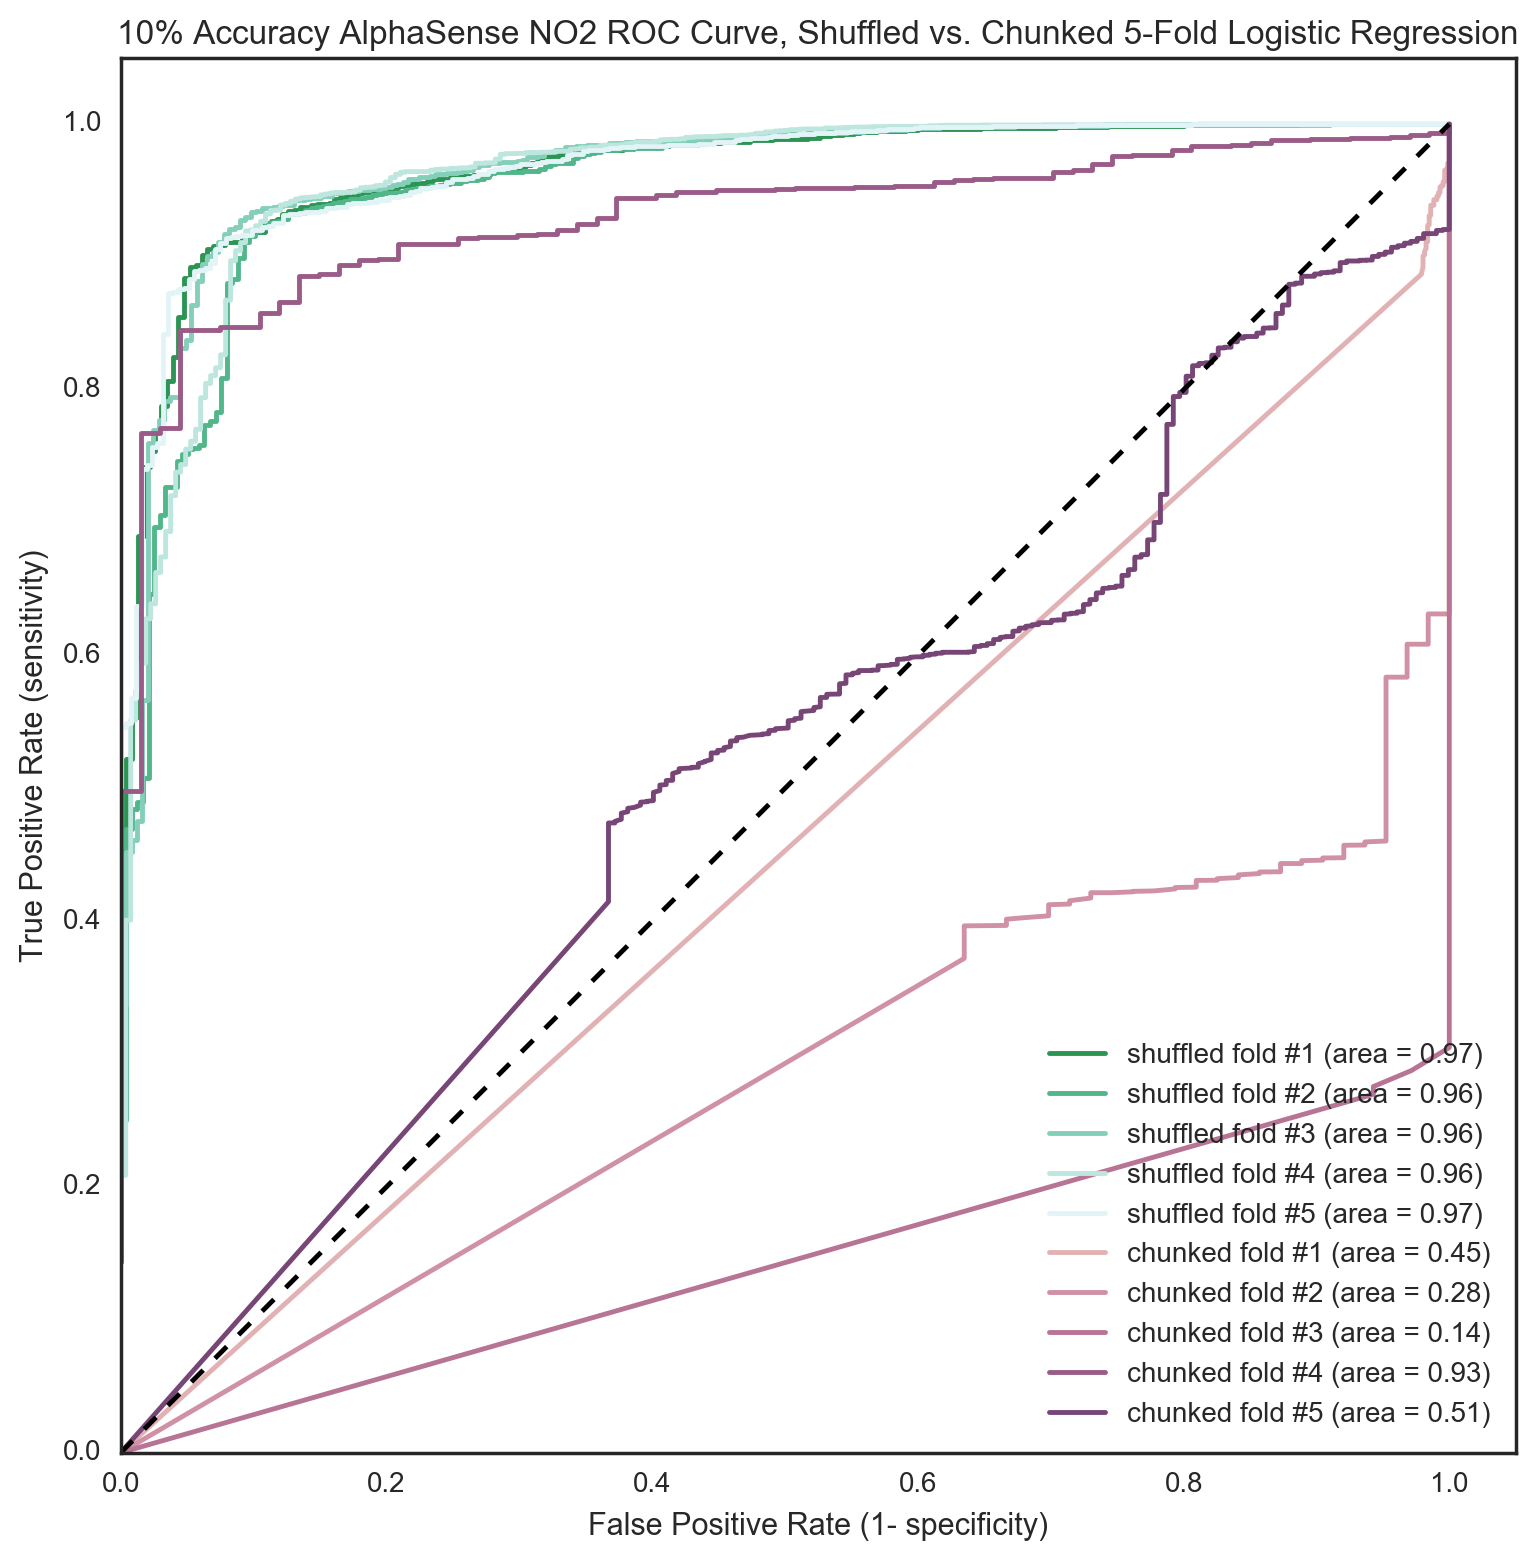
\includegraphics[width=\textwidth]{figs/as_no2_10_roc}               
 	 \caption{AlphaSense NO2 ROC Curve}
  	\label{fig:as_no2_10_roc}
\end{figure}


The top features  (Table \ref{tab:as_no2_top_features}) and the effect of reducing the feature set aren't particularly meaningful given our prior conclusion, but the fact that black carbon, cloud cover, and O3 concentration are in the top several features (and these features seem to do a good job predicting robustness in the shuffled case by themselves) bolsters the hypothesis that there is likely a useful, predictable trend underlying this data.  We would expect our high quality correlated sensor to provide a good backbone for prediction, and cloud cover and O3 directly point to one of the most rapid and important reactions that converts NO2 to other by-products.  Since these highly relevant features drive our strong shuffled predictions (as oppose to spurious, coincidental ones),  it seems likely that this AlphaSense NO2 sensor will be highly predictable with a few more weeks of data collection.

\begin{table}[]
\centering
\small
\begin{tabular}{lllllllll}
\\
\\
\toprule
     & Corr. & Lasso & Lin Reg & RF   & RFE  & Ridge & Stability & Mean \\
\midrule
bkcarbon                          & 0.99  & 0     & 0          & 0.85 & 0.47 & 0.23  & 0.79      & 0.48 \\
avg\_60\_bkcarbon                 & 1     & 0     & 0          & 1    & 0.54 & 0.14  & 0.64      & 0.47 \\
avg\_1440\_bkcarbon               & 0.9   & 0     & 0          & 0.16 & 0.5  & 0.44  & 0.69      & 0.38 \\
daily\_avg\_sck\_humidity         & 0.36  & 0     & 0          & 0.03 & 0.59 & 0.77  & 0.39      & 0.31 \\
as\_o3                            & 0.02  & 0     & 0          & 0.97 & 0.77 & 0.01  & 0.42      & 0.31 \\
lmse\_sck\_co                     & 0.06  & 1     & 0          & 0.01 & 0.81 & 0     & 0.28      & 0.31 \\
avg\_60\_forecastio\_cloudCover   & 0.16  & 0     & 0          & 0.11 & 0.53 & 0.38  & 0.81      & 0.28 \\
Solar Panel ( V)                  & 0.05  & 0     & 1          & 0    & 0.87 & 0     & 0         & 0.27 \\
derivative\_avg\_1440\_bkcarbon   & 0.17  & 0     & 0          & 0.04 & 0.62 & 0.08  & 1         & 0.27 \\
sck\_humidity\_saturated          & 0.04  & 0     & 0          & 0.01 & 0.58 & 1     & 0         & 0.23 \\
avg\_720\_lmse\_scaled\_sharpDust & 0     & 0     & 0          & 0.37 & 0.57 & 0.67  & 0.01      & 0.23 \\
avg\_720\_bkcarbon                & 0.85  & 0     & 0          & 0.2  & 0.16 & 0.06  & 0.35      & 0.23 \\
evening                           & 0.05  & 0     & 0          & 0    & 0.95 & 0.04  & 0.47      & 0.22 \\
day                               & 0.06  & 0     & 0          & 0    & 0.99 & 0.06  & 0.42      & 0.22 \\
night                             & 0.06  & 0     & 0          & 0    & 1    & 0.06  & 0.41      & 0.22 \\
alphaS2\_work                     & 0.31  & 0.78  & 0          & 0.02 & 0.21 & 0.05  & 0.09      & 0.21 \\
forecastio\_fog                   & 0.05  & 0     & 0.4        & 0    & 0.93 & 0     & 0         & 0.2  \\
forecastio\_temperature\_c        & 0     & 0     & 0.01       & 0    & 0.93 & 0.01  & 0.44      & 0.2  \\
derivative\_avg\_720\_bkcarbon    & 0.09  & 0     & 0          & 0.05 & 0.61 & 0.15  & 0.5       & 0.2  \\
forecastio\_temperature           & 0     & 0     & 0          & 0    & 0.92 & 0.01  & 0.41      & 0.19 \\
Carbon Monxide ( kOhm)            & 0.06  & 0     & 0          & 0.01 & 0.82 & 0     & 0.34      & 0.18 \\
forecastio\_cloudCover            & 0.19  & 0     & 0          & 0.01 & 0.44 & 0.17  & 0.48      & 0.18 \\
forecastio\_partly-cloudy-day     & 0.05  & 0     & 0.04       & 0    & 0.89 & 0.01  & 0.23      & 0.17 \\
\bottomrule
\end{tabular}
\label{tab:as_no2_top_features}
\caption{Top Features for Predicting AlphaSense NO2}
\end{table}
